\chapter{Entropy Generation and Exergy Analysis}\label{ch:exergy}

\section{Entropy Generation Formulation}
Local entropy generation density is approximated by
\begin{equation}\label{eq:entropy_local}
\dot{s}_{gen}=\frac{k_{eff}}{T^2}(\nabla T)^2+\frac{\mathbf{J}_e^2}{\sigma_{eff}T}+\frac{q''\Delta T_{int}}{T^2}.
\end{equation}
Volume-integrated entropy generation rate:
\begin{equation}\label{eq:entropy_total}
\dot{S}_{gen}=\int_V \dot{s}_{gen}\,\mathrm{d}V.
\end{equation}
Bejan number is
\begin{equation}\label{eq:bejan}
Be=\frac{\dot{S}_{gen,heat}}{\dot{S}_{gen,heat}+\dot{S}_{gen,joule}+\dot{S}_{gen,int}}.
\end{equation}

\section{Exergy Efficiency}
Thermal exergy input over a cycle is
\begin{equation}\label{eq:ex_in}
\dot{E}_{x,in}=\dot{Q}_{in}\left(1-\frac{T_0}{T_h}\right).
\end{equation}
Useful exergy output is electrical power $\dot{W}_{el}$. Thus
\begin{equation}\label{eq:ex_eff}
\eta_{ex}=\frac{\langle \dot{W}_{el}\rangle}{\langle \dot{E}_{x,in}\rangle}.
\end{equation}
Exergy destruction is
\begin{equation}\label{eq:ex_dest}
\dot{E}_{x,d}=T_0\dot{S}_{gen}.
\end{equation}

\section{Optimization Insight}
A scalar optimization objective is
\begin{equation}\label{eq:objective}
\max\,\mathcal{J}=w_1\eta_{ex}+w_2\Psi-w_3D_N.
\end{equation}
This identifies balanced designs where thermal buffering and transport enhancement outweigh durability penalties.

\begin{figure}[htbp]
\centering
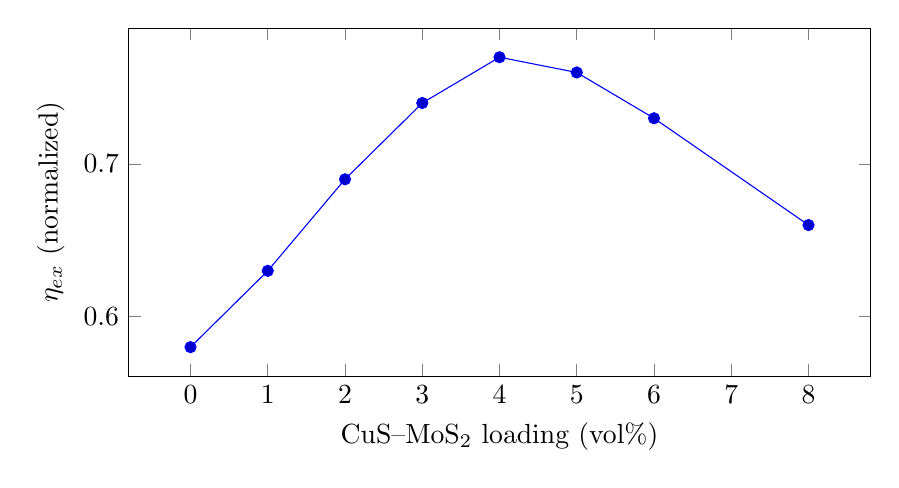
\begin{tikzpicture}
\begin{axis}[width=11cm,height=6cm,xlabel={CuS--MoS$_2$ loading (vol\%)},ylabel={$\eta_{ex}$ (normalized)}]
\addplot+[mark=*] coordinates {(0,0.58)(1,0.63)(2,0.69)(3,0.74)(4,0.77)(5,0.76)(6,0.73)(8,0.66)};
\end{axis}
\end{tikzpicture}
\caption{Exergy efficiency versus reinforcement loading showing a distinct optimum.}
\label{fig:exergy_loading}
\end{figure}

\begin{table}[htbp]
\centering
\caption{Entropy generation decomposition (normalized values).}
\label{tab:entropy_split}
\begin{tabular}{lccc}
\toprule
Design & Heat-transfer term & Joule term & Interfacial term \\
\midrule
Baseline & 0.51 & 0.34 & 0.15 \\
Optimized hybrid & 0.44 & 0.31 & 0.12 \\
Overfilled filler & 0.46 & 0.33 & 0.21 \\
\bottomrule
\end{tabular}
\end{table}
